%%%%%%%%%%%%%%%%%%%%%%%%%%%%%%%%%%%%%%%%%%%%%%%%%%%%%%%%%%%%%%%%%%%%%%%%%%%%%%%%
%							IMPLEMENTING ERM WITH DNN						   %
%%%%%%%%%%%%%%%%%%%%%%%%%%%%%%%%%%%%%%%%%%%%%%%%%%%%%%%%%%%%%%%%%%%%%%%%%%%%%%%%
As we have seen, the hypothesis class of \glspl{dnn} is fully defined by the \glspl{hp} describing the architecture, whereas a specific instance \(\MLmodel\) of neural network among \(\hypoclass\) is also defined by the vector \(\MLparam\) of all the learning parameters.
In other words, one can re-write a model from \(\hypoclass\) under the form \(\fonction{\MLmodel}{\cdot, \MLparam}\).
As a consequence, implementing the \gls{erm} principle can be translated from a functional optimization perspective -- \ie{} finding the model \(\MLmodel \in \hypoclass\) minimizing the training loss -- into a numerical optimization problem -- \ie{} finding the vector \(\MLparam\) such that the function \(\MLmodel(\cdot, \MLparam)\) minimizes the training loss.
Since closed-form solutions do not exist, this numerical optimization problem is usually solved thanks to an iterative optimization algorithm such as \gls{sgd}%
\footnote{
	We recall that \autoref{sec:optim_algo} introduced the \gls{sgd} algorithm.
} 
by iteratively updating the values of the learning parameter \(\MLparam\), as illustrated in \autoref{fig:schema_dnn_sgd}.
\tikzset{
		>=stealth',
	    %BASE STYLE
	    base/.style = {minimum height=0.1cm,
	                   minimum width=0.2cm,
	                   text centered,
	                   font=\sffamily},
	    %ROUNDED STYLE
	    rounded/.style = {base,
	                      rounded corners},
}
\begin{figure}
	\centering
	\begin{tikzpicture}[scale=0.2]
		\node (Chip) {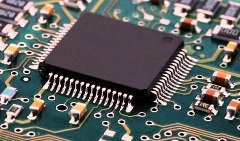
\includegraphics[width=0.1 \textwidth]{illustrations/chip}};
		\node[right = of Chip] (Scope) {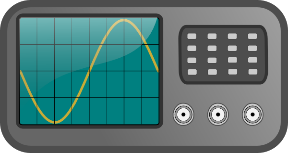
\includegraphics[width=0.1 \textwidth]{illustrations/scope}};
		\node[above right = of Chip] (PC) {
\includegraphics[width=0.1 \textwidth]{illustrations/pc}};
		\node[right = of Scope] (Trace) {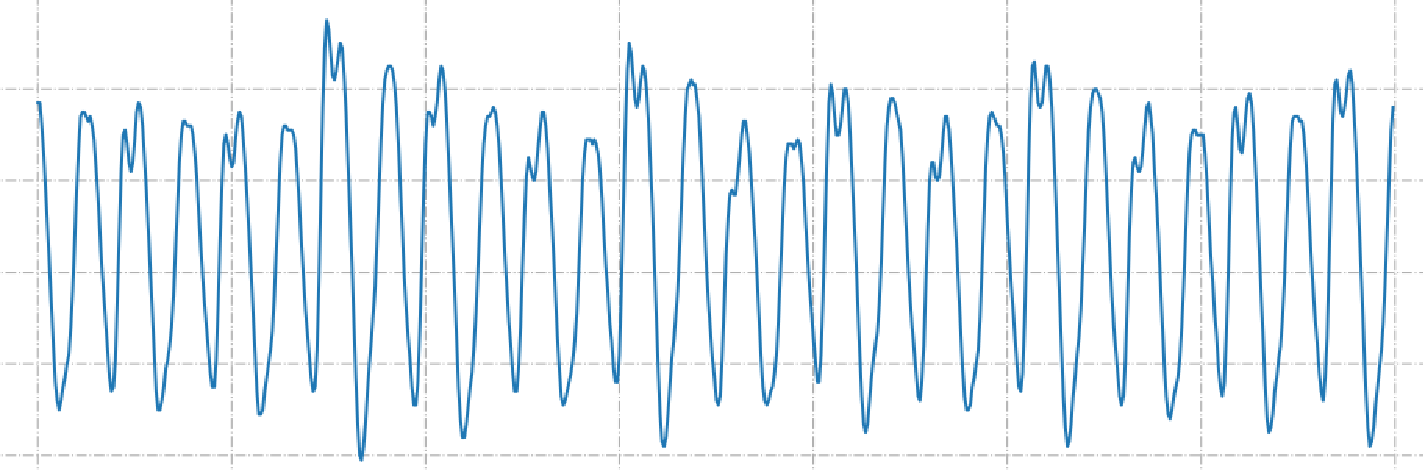
\includegraphics[width=0.2 \textwidth,angle=90]{illustrations/trace}\(\xxx\)};
		\node[rounded, fill=ceablue!30, right = of Trace] (Model) {\small \(\MLmodel(\xxx, \MLparam)\)};
		\node[right = of Model] (Scores) {
\includegraphics[width=0.2 \textwidth,angle=90]{illustrations/scores}};
		\node[rounded, fill=ceared!30, below = of Model] (Param) {\small Parameters \(\MLparam\)};
		\node[rounded, fill=ceadarkred!30, right = of PC] (Z) {\small \(\z = \miniEncrypt{\p, \keyTest}\)};


		\node[rounded, fill=cealime!30, right = of Scores] (Loss) {\small \(\lossFunc{\vNNOutput, \z}\)};

		\draw[->] (Chip)  -- (Scope);
		\draw[->] (Chip)  -- (PC);
		\draw[->] (Scope) -- (Trace);
		\draw[->] (PC)    -- (Z);
		\draw[->] (Trace) -- (Model);
		\draw[->] (Param) -- (Model);
		\draw[->] (Model) -- (Scores);

		\draw[->] (Scores) -- (Loss);
		\draw[->] (Z) -| (Loss);
		\draw[->] (Loss) |- (Param);
	\end{tikzpicture}
	\caption{Illustration of the workflow of the training of a \gls{dnn} in a profiled \gls{sca} context.}
	\label{fig:schema_dnn_sgd}
\end{figure}

Interestingly, the \gls{erm} principle introduced by the \gls{ml} framework remains a purely theoretical tool in most of the applications, and particularly in deep learning.
Indeed, it often cannot be implemented in practice, for several reasons that we will describe in the following subsections.
Finally, we explain in \autoref{sec:computing_gradient} how the derivatives of the loss function, a crucial element required by the optimization algorithm, is efficiently computed.
This description will serve as a discussion in \autoref{chap:gradient_viz}.


\subsection{\gls{sca} Metrics are Hard to Optimize}
\label{sec:erm_hard}
So far in this chapter, we have presented the \gls{ml} framework for a generic learning problem.
In particular, we have considered so far an abstract loss function \(\lossFunc{}\) to minimize, whose generic definition has been given in \autoref{eq:loss_function}.
It is indeed tempting at first sight to use the final performance metric as a loss function, in order to guarantee the convergence of the trained model towards the best possible one, according to \autoref{thm:consistency}.
Unfortunately, one cannot optimize with respect to any loss function, regardless the underlying hypothesis class \(\hypoclass\).

For example, in supervised classification the ultimate performance metric is the \emph{accuracy}, namely the rate of accurate predictions among the possible labels that may be recognized by the model.
% Definition
For any function \(\MLmodel: \leakSpace \rightarrow \realSet^{\card{\sensVarSet}}\), the accuracy is denoted by \(\acc_{\XXX, \Z}(\MLmodel)\) and is defined as:
\begin{equation}
	\acc_{\XXX, \Z}(\MLmodel) \eqdef \prob{\argmax_{\sensValue \in \sensVarSet}\MLmodel(\XXX)[s] = \Z} 
	 = \esper[\XXX, \Z]{\charac{\argmax_{\sensValue \in \sensVarSet}\MLmodel(\XXX)[s] = \Z}}
	\enspace .
\end{equation}
That is, this metric gives the rate of right predictions, or more precisely the probability that the highest score returned by a learning algorithm based on a single input data \(\XXX\) corresponds to the class \(\Z\) it is assigned.
Therefore, maximizing the accuracy is suitable to address the \emph{classification} task.

% NP-hard
Unfortunately, solving the \gls{erm} for \glspl{dnn} with the accuracy as a loss function turns out to be \gls{nph}~\cite[Sec.~20.5]{shalev-shwartz_understanding_2014}.
In a nutshell, the reason comes from the fact that the resulting training loss can be formulated as a sum of characteristic functions:%
\footnote{
	See \autoref{sec:notations} for a definition of a characteristic function.
}
\begin{equation}
	\acc_{\trainSet}(\MLmodel) \eqdef \frac{1}{\card{\trainSet}} \sum_{\xxx, \z \in \trainSet} \charac{\argmax_{\sensValue \in \sensVarSet}\MLmodel(\xxx)[s] = \z} \enspace .
	\label{eq:acc_charac}
\end{equation}
Each characteristic function in \autoref{eq:acc_charac} has null derivatives \gls{ae}, and so has the training loss of the accuracy, as depicted in \autoref{fig:example_acc} with the staged red curve depicting the training loss, as a sum of characteristic functions.
So gradient-descent-based optimization algorithms are useless, and no other efficient alternative could circumvent this issue.
\begin{figure}
	\centering
	\begin{tikzpicture}
		\begin{axis}[thick,axis x line=bottom, axis y line=left, no markers, xlabel = {\(\MLparam\)}, xtick=\empty, ytick=\empty, every axis x label/.style={at={(current axis.right of origin)}, anchor=north west}, legend pos=outer north east]
			\addplot[ceablue] {x^2};
			\addlegendentry{\(\LossFunc[\XXX, \Z]{\MLparam}\)}
			\addplot[samples=200, ceadarkred] {(round(2*x)/2)^2};
			\addlegendentry{\(\LossFunc[\trainSet]{\MLparam}\)}
		\end{axis}
	\end{tikzpicture}
	\caption{Toy example of a training loss made of characteristic functions with respect to a real valued learning parameter \(\MLparam\).
	Paradoxically, although the training loss \(\LossFunc[\trainSet]{\MLparam}\) has zero derivatives \gls{ae}, the generalization loss \(\LossFunc[\XXX, \Z]{\MLparam}\) may have non-null derivatives.}
	\label{fig:example_acc}
\end{figure}

% Classification -> SCA
Interestingly, this drawback also concerns the efficiency \(\MLmodel \mapsto \numTracesAttack(\MLmodel)\), defined in \autoref{sec:performance_metrics} as the minimal number of attack traces to succeed the attack beyond a probability threshold \(\beta\) fixed by the evaluator, and that we chose as an ultimate performance metric according to \autoref{final_task_prof}.
The corresponding training loss to minimize in the \gls{erm} would depend on the guessing vector defined in \autoref{eq:guess_vec}.
But the latter quantity is a sum of characteristic functions, hence meeting the same issues as the training loss corresponding to accuracy.
That is why the \gls{sca} metrics are hard to directly optimize.

% Other learning algorithms
More generally, this also holds for Random Forest and \glspl{svm}, two other learning algorithms used in the \gls{sca} literature~\cite{picek_curse_2019}: the former one is based on heuristics working reasonably well in practice~\cite[Chap.~18.2]{shalev-shwartz_understanding_2014} whereas the latter one must minimize another loss function called \emph{Hinge} loss~\cite[Chap.~15.2.3]{shalev-shwartz_understanding_2014}.

\subsection{The Need for a Surrogate Loss}
\label{sec:surrogate_loss}
The previous section raises the need for a suitable \emph{surrogate} loss function, either found among the usual functions considered in the \gls{dl} literature, or designed specifically for our problem.
In the literature, mostly two surrogate loss functions have been used in the \gls{sca} context: the \glsfirst{nll}~\cite{cagli_convolutional_2017,prouff_study_2018,kim_make_2019} and the \gls{mse}%
\footnote{
	From a purely optimization point of view, the \gls{mse} might suffer from problems~\cite{nielsen_neural_2018}.
	From a \gls{sca} evaluation point of view, the relevance of \gls{mse} is an open question~\cite{picek_bias_2019}, beyond the scope of this thesis.
}~\cite{maghrebi_breaking_2016, timon_non-profiled_2019,wegener_dlla_2019}.
Until a few years ago, nobody particularly raised the issue into the \gls{sca} community since the empirical results obtained for any loss function on several use cases got promising results from an attacker's point of view.
Nevertheless, from an evaluator's point-of-view, it remains necessary to assess whether the problem of minimizing the chosen training loss is actually equivalent to the profiled \gls{sca} optimization problem.
More precisely, whether:
\begin{enumerate}
	\item both problems share the same analytical optimal solution \(\MLmodel^\star\);
	\item improving a sub-optimal solution for one problem directly leads to get an improved sub-optimal solution for the other one.
\end{enumerate}
Tackling this issue is of great interest in \gls{sca}.
Indeed nowadays there might still be a gap between the recent practical successes of this class of attacks, and the theoretical soundness of \gls{dl}-based \gls{sca}: what is the sense of training a \gls{dnn} by minimizing a surrogate loss function from an \gls{sca} point of view?
This issue will be at the core of \autoref{chap:ches_20}.

\subsection{The Challenge of Optimization}
\label{sec:challenge_optimization}
We have seen that the interest of the surrogate loss function is to be differentiable with respect to all the learning parameters,%
\footnote{
	We recall that the parameters describing the architecture for which the loss is not differentiable are called \emph{\glspl{hp}}.
} 
in order to use a gradient based optimization algorithm such as \gls{sgd}.
Nevertheless, in \gls{dl}, this still raises an important issue, even when using a surrogate loss. 
Indeed, when considering the specific hypothesis class of \glspl{dnn}, the resulting \emph{objective}%
\footnote{
	The term ``objective'' function is the terminology used by the numerical optimization research community.
	It refers to the training loss function in the specific case of machine learning.
	In the following, we will rather use the term ``loss'' to design the function to minimize.
} 
function to optimize is shown to be highly non-convex~\cite{choromanska_loss_2015}, contrary to \glspl{svm} whose surrogate loss, \ie{} Hinge loss, spans a convex optimization problem.
Moreover, the solution to the problem is not unique: considering one \gls{dnn} model minimizing the training loss, the same model whose entries of the intermediate layers are permuted -- and so are the learning parameters accordingly -- would return the same result.
Hence, the number of equivalent solutions is \emph{combinatorial} with respect to the output size of the intermediate layers of the model.

As a consequence, the usual numerical optimization algorithms are not theoretically guaranteed to converge towards an optimal solution, which prevents the \gls{sgd} algorithm and its variants to perfectly instantiate the \gls{erm} principle.
In other words, the optimization error cannot be assumed to be negligible, as already discussed in \autoref{sec:erm_principle}.
Nevertheless, experience has surprisingly shown that those algorithms represent a satisfying heuristic~\cite{lecun_efficient_2012}, and the recent literature started to provide theoretical insights about this fact~\cite{du_gradient_2019,du_gradient2_2019}.

\subsection{Computing the Gradient}
\label{sec:computing_gradient}
So far in this section, we have explained that the \gls{erm} principle could be implemented by addressing a non-convex numerical optimization problem.
We explained in the previous sections to what extent perfectly solving this problem is hard in practice, although sound approximate solutions could be returned by an optimization algorithm such as the \gls{sgd}.
The latter algorithm -- and its variants -- rely on the computation of \emph{descent} directions based on the gradient of the loss function defined in \autoref{eq:empirical_loss} and computed with respect to the parameter vector, namely \(\grad[\MLparam]{\LossFunc[\trainSet]{\MLmodel(\cdot, \MLparam)}}\).
It is therefore of great interest to study to what extent providing the gradient of the loss function to the optimization algorithm is affordable when considering models from the hypothesis class of \glspl{dnn}.
This subsection is devoted to this discussion.
\begin{remark}
	The details provided in this subsection concern more generally any \gls{dl}-based problem, and not only \gls{sca}.
	Nevertheless, it will be useful for future discussions in \autoref{chap:gradient_viz}.
\end{remark}
The training loss to minimize being a sum of elementary losses over the profiling set, so is the gradient:
\begin{equation}
	\grad[\MLparam]{\LossFunc[\trainSet]{\MLmodel(\cdot, \MLparam)}} = 
	\frac{1}{\numTracesProf} \sum_{i=1}^{\numTracesProf} \grad[\MLparam]{\lossFunc{\MLmodel(\xxx_i, \MLparam), \z_i}} \enspace .
	\label{eq:grad_empirical_loss}
\end{equation}
It turns out that an algorithm called \emph{backward propagation} (\aka{} backprop) can exactly compute the gradient of \(\lossFunc{\MLmodel(\xxx_i, \MLparam), \z_i}\) with respect to \(\MLparam\) for roughly the same complexity of computing \(\lossFunc{\MLmodel(\xxx_i, \MLparam), \z_i}\) itself.
It relies on the use of the chaining rule recalled in \autoref{lemma:chaining_rule}.
Indeed, due to the layer-wise nature of \(\MLmodel(\cdot, \MLparam)\), the loss function, seen as a function of the parameter vector \(\MLparam\), can also be seen as a sequence of compositions of elementary functions whose derivatives can be computed in a closed-form solution.
Therefore, by using recursively the chaining rule on the given sequence of functions, one is able to exhibit an efficient procedure to exactly compute the gradient.

It is noticeable that for a composition of \(n > 2\) elementary functions, the chaining rule can be recursively applied in two manners, respectively denoted as \emph{forward} and \emph{reverse}.
We explain hereafter the stakes behind those two automatic differentiation modes on an example of compositions of \(n\) elementary functions \((f_i)_{1 \leq i \leq n}\) such that:
\begin{equation}
	f_i: \realSet^{m_{i-1}} \rightarrow \realSet^{m_i} \enspace ,
\end{equation}
where \(m_i \geq 1\) for \(0 \leq i \leq n-1\), \(m_{n-1} = \card{\sensVarSet}\), and \(m_n = 1\).
The resulting function to differentiate \(\ell: \realSet^{m_n}\rightarrow \realSet\) can then be written as:
\begin{equation}
	\lossFunc{\MLparam} = 
	\lefteqn{\overbrace{\phantom{f_n \circ \ldots \circ f_i}}^{\varphi_{n-i} \mbox{\tiny (Reverse)}}}
	f_n \circ \ldots \circ 
	\underbrace{f_i \circ \ldots \circ f_1}_{\psi_i \mbox{\tiny (Forward)}}
	\label{eq:autodiff_mode}
\end{equation}
We recall furthermore that the elementary functions \((f_i)_{1 \leq i \leq n}\) are assumed to be simple enough to derive closed-form expressions of their \glspl{jacob}.

% Forward mode
In a \emph{forward} mode, the chaining rule is applied from right to left%
\footnote{
	We draw the attention of the reader on the fact that when composing several functions, the notation \(f_2 \circ f_1\) must be read backward, hence ``forward'' means here ``right-to-left''.
} 
in \autoref{eq:autodiff_mode}.
That is, by considering the sequence of mappings defined by \(\psi_0 = I_d\) the identity mapping and \(\psi_{i+1} = f_{i+1} \circ \psi_i, \enspace 0 \leq i \leq n-1\), and by applying \autoref{lemma:chaining_rule}, it follows that:
\begin{equation}
	\underbrace{\jac{\psi_{i+1}}{\MLparam}}_{(m_{i+1}, m_0)} = \underbrace{\jac{f_i}{\psi_i(\MLparam)}}_{(m_{i+1}, m_i)} \cdot \underbrace{\jac{\psi_i}{\MLparam}}_{(m_i, m_0)}
	\label{eq:forward_mode}
\end{equation}
Since one remarks that \(\psi_n(\MLparam) = \lossFunc{\MLparam}\), it is then possible to compute its gradient by iteratively applying \autoref{eq:forward_mode}.
But this method requires to store the \glspl{jacob} of the mappings \(\psi_i\) whose sizes are respectively \(m_i \times m_0\), which might be prohibitive if the intermediate outputs are of high dimensionality.

% Reverse mode
In a \emph{reverse} mode, the chaining rule is applied from left to right in \autoref{eq:autodiff_mode}.
That is, by considering the sequence of mappings defined by \(\varphi_1 = f_n\) and \(\varphi_{i+1} = \varphi_i \circ f_{n-i}, \enspace 1 \leq i \leq n-1\), and by applying \autoref{lemma:chaining_rule}, it follows that for every \(\xxx \in \realSet^{m_{n-i}}\):
\begin{equation}
	\jac{\varphi_{i+1}}{\xxx} = 
	\jac{\varphi_i}{f_{n-i}(\xxx)} \cdot 
	\jac{f_{n-i}}{\xxx}
\end{equation}
By taking \(\xxx = \psi_{n-(i+1)}(\MLparam)\), it follows that:
\begin{equation}
	\underbrace{\jac{\varphi_{i+1}}{\psi_{n-(i+1)}(\MLparam)}}_{(1, m_{n-i})} = 
	\underbrace{\jac{\varphi_i}{\psi_{n-i}(\MLparam)}}_{(1, m_{n-i-1})} \cdot 
	\underbrace{\jac{f_{n-i}}{\psi_{n-(i+1)}(\MLparam)}}_{(m_{n-i-1}, m_{n-i})}
	\label{eq:reverse_mode}
\end{equation}
Since one remarks that \(\varphi_n = \ell\) it is here again possible to compute its gradient by iteratively applying \autoref{eq:reverse_mode}.
Yet, compared to the forward mode, two main differences should be noticed.
% First diff: need for a forward pass before differenciating
First, it is necessary to store all the intermediate computations \(\left(\psi_i(\MLparam)\right)_{1 \leq i \leq n}\) when previously computing the loss function \(\lossFunc{\MLparam}\), whereas in a forward mode the gradient can be directly computed without necessarily computing \(\lossFunc{\MLparam}\).
% Second diff: one only store 1 gradient instead of 1 jacobian matrix
Second, rather than storing a \gls{jacob} after each iteration, the reverse mode enables to only store a gradient of size \(m_{n-i}\), which is much lighter than in the forward mode.
That is why all the \glspl{api} devoted to \glspl{dnn} only use the reverse mode in their implementations, and are optimized in order to avoid the storage of any \gls{jacob}, hence the name of ``backprop'' which explicitly refers to the ``reverse'' mode.
This point will be later discussed in \autoref{chap:gradient_viz}.

% Biblio
The backprop algorithm has been independently discovered many times during the 70's and the 80's, in particular by Hinton \etal{} in 1986~\cite{rumelhart_learning_1986,hinton_backprop_1986}.
More generally, the backprop algorithm has paved the way towards \emph{automatic differentiation} which studies how to efficiently differentiate functions \emph{numerically},%
\footnote{
	\ie{} in opposition to \emph{symbolic} differentiation considering only algebraic formulations of a function.
} 
which is often crucial in machine learning.
The interested reader may refer to the survey of Baydin \etal{}~\cite{baydin_automatic_2017}.

\subsection{Some \glspl{api}}
\label{sec:apis}
Training \glspl{dnn} with optimization algorithms is nothing but linear algebra computations -- \eg{} scalar and matrix product -- in very high dimensionality, typically \(10^5 - 10^6\).
To scale with this range, the implementation must leverage massively parallel programming, either in \gls{cpu} clusters of on \glspl{gpu}.
That is why until few years ago, the \gls{ml} practitioners used to need strong skills in a broad spectrum of programming fields.
Those skills were hard to gather into a research team, and most of the time of researchers was devoted to implementing models which were not easily reproducible by the scientific community.

% APIs in Deep Learning
That is why, with the emergence of deep learning in the beginning of the 2010's, several \glspl{api} have been released by the machine learning community.
Although the very first public library \textsf{Theano}~\cite{theano} is not maintained anymore by its authors, several other \glspl{api} have been publicly developed over the last few years, such as \textsf{Pytorch}~\cite{pytorch_2019}, supported by Facebook; \textsf{Tensorflow}~\cite{tensorflow2015-whitepaper}, supported by Google; or \textsf{Keras}~\cite{chollet2015keras}, an extension of \textsf{Tensorflow} initiated by Chollet.
In particular, the source code developed for this thesis has been written in \textsf{Python} with the help of the \textsf{Pytorch} \gls{api},%
\footnote{The library is available at \url{pytorch.org}.}
and is run on a workstation with a \textsf{Nvidia Quadro M4000} \gls{gpu} with 8 GB memory and 1664 cores, and 32~GB of \gls{ram}.

\subsection{On the Accuracy as a Monitoring Metric}
\label{sec:issue_accuracy}
We have seen in \autoref{sec:erm_hard} that in supervised classification, it is not possible to directly maximize the accuracy of \glspl{dnn}, since it is a \gls{nph} problem.
Despite its impossibility to directly minimize, most of the works considering \gls{dl}-based \gls{sca} made use, explicitly or implicitly, of the accuracy as a monitoring metric, assuming that such a performance measure may still be informative of the quality of a trained model.

Cagli \etal{}~\cite{cagli_convolutional_2017} and Picek \etal{}~\cite{picek_curse_2019} were the first to raise this issue, namely the relevance of the \emph{accuracy}, a widely used \gls{ml} performance metric, in the context of \gls{sca}.
Unfortunately, we explain hereafter that it is not the case.

It turns out that the optimal model for \gls{sca}, which is \(\MLmodel^{\star} = \prob{\Z \given \XXX}\), is also the optimal classifier for the supervised classification task.%
\footnote{
	The \gls{ml} literature often uses the term \emph{Bayes' classifier} to denote the optimal classifier for the classification task.
} 
This means that for any function \(\MLmodel: \leakSpace \rightarrow \probSet{\sensVarSet}\) we have:
\begin{equation}
	\acc(\MLmodel) \leq \acc(\MLmodel^{\star}) \enspace .
\end{equation}
In other words, both supervised classification problem and \autoref{final_task_prof} share the same analytical optimal solution \(\MLmodel^\star\), which is the first of the two conditions stated in \autoref{sec:surrogate_loss} to get a loss function equivalent to our \gls{sca} efficiency metric.
Thus, the accuracy might be a good metric candidate.
Yet, both problems sharing the same optimal solution \(\MLmodel^\star\) does not necessarily mean that they are equivalent, since it remains to verify that improving sub-optimal solutions for one problem should lead to improved sub-optimal solutions for the other.

Cagli \etal{}\,recalled that the accuracy could be translated into another \gls{sca} metric, namely the success rate when recovering the key with one trace \(\succRate(1)\).
In a sense, \(\acc(\MLmodel)\) is the \emph{dual} metric of \(\numTracesAttack(\MLmodel, 1, \beta)\): the former one fixes \(\numTracesAttack=1\) and estimates the corresponding threshold \(\beta\), whereas the latter one fixes the threshold and estimates the minimum value \(\numTracesAttack\) such that \(\succRate(\numTracesAttack, \MLMLEscore{\attackSet}{\MLmodel}, 1) \geq \beta\) -- see \autoref{eq:SR}.
Cagli \etal{}\,have emphasized that although this could have a sense in some specific scenarios, \eg{}, when evaluating implementations of asymmetric cryptographic primitives, this does not necessarily have a sense to evaluate the robustness of a target against an attack involving only one trace.
That is why at first sight, accuracy does not seem appropriate in our context.

Picek \etal{} empirically confirmed a similar observation at \textsc{Ches}'19~\cite{picek_curse_2019}.
For several learning algorithms, such as \glspl{svm} and Random Forests, they empirically compared the obtained \gls{ge} with the accuracy, and they found out that there is no clear link between them.
More precisely, they argue that a high accuracy -- \ie{}, with respect to the one obtained with a model providing completely random predictions -- is a clue for effective attacks, though the inverse does not empirically hold: a low accuracy does not necessarily imply a failed key recovery.
However, the latter case may often happen, especially with protected implementations where the noise artificially induced by the counter-measures reduces the performances of the optimal model, and so the accuracy.

As a conclusion to the two latter sections, the accuracy is not only useless for the implementation of the \gls{erm}, as already concluded in the end of \autoref{sec:erm_hard}, but is also a poor metric to monitor in an \gls{sca} context.
Recently, new ways to monitor the quality of a \gls{dnn} have been proposed, in particular by Robissout \etal{}~\cite{robissout_online_2020} and Perin \etal{}~\cite{perin_learning_2020}.
Although this brings new insights, those monitoring metrics partially circumvent the problems raised by the accuracy, since the metrics proposed there are not optimizable.
Finding a proper loss function which is useful not only as a quantity to optimize but also as a metric to monitor is the core problem which will be addressed in \autoref{chap:ches_20}.